%*****************************************
\chapter{Deep Learning and Generative Models}\label{ch:dlgm}
%*****************************************
%Acronym testing: \ac{UML} -- \acs{UML} -- \acf{UML} -- \acp{UML}

In recent years, \emph{machine learning} techniques have been massively adopted by scientific collaboration around the world. In particular, a paradigm known as \emph{Deep Learning}, which leverages multiple layers of \emph{artificial neurons} trained through the use of a \emph{loss function} and \emph{backpropagation}, has achieved a wide range of applications.

The present chapter will give to the reader a concise but hopefully complete overview of the building blocks behind the recent success of Deep Learning. A great introduction, which served the writer well in its own approach to the field, is the one by Michael Nielsen \cite{nielsenneural}. Towards the conclusion we turn to the class of \emph{generative models}, paving the way for the next chapter discussion.
	

\section{Neural Networks}

The name \emph{neural networks} can be understood as a beautiful biologically-inspired programming paradigm, which enables a computer to learn from data. The main idea is (or at least \emph{was}, initially) to emulate how our brains work. In particular, this requires a modelling of the basic brain unit, the neuron, and of its interactions with neighboring units.

\subsection{The Perceptron}

One of the earliest implementation of an algorithm inspired  by our biological brains is due to Rosenblatt \cite{Rosenblatt1958ThePA}. Its \emph{Perceptron} is a type of artificial neuron working exclusively on binary inputs. This scheme mimics the firing of neurons to transmit electrical signals along synapses.

The architecture is illustrated in Figure \ref{fig:rosper}.

\begin{figure}
    \centering
    
    \begin{tikzpicture}
        \node[functions] (left){};
            \node[right = 1.0cm of left] (right) {$y$};
            \path[draw,->] (left) -- (right);
        \node[left=3em of left] (2) {$w_2$} -- (2) node[left of=2] (l2) {$x_2$};
            \path[draw,->] (l2) -- (2);
            \path[draw,->] (2) -- (left);
        \node[below of=2] (dots) {$\vdots$} -- (dots) node[left of=dots] (ldots) {$\vdots$};
        \node[below of=dots] (n) {$w_n$} -- (n) node[left of=n] (ln) {$x_n$};
            \path[draw,->] (ln) -- (n);
            \path[draw,->] (n) -- (left);
        \node[above of=2] (1) {$w_1$} -- (1) node[left of=1] (l1) {$x_1$};
            \path[draw,->] (l1) -- (1);
            \path[draw,->] (1) -- (left);
        \node[above of=1] (0) {$w_0$} -- (0) node[left of=0] (l0) {$1$};
            \path[draw,->] (l0) -- (0);
            \path[draw,->] (0) -- (left);
        \node[above of=l0,font=\scriptsize] {inputs};
        \node[above of=0,font=\scriptsize] {weights};
    \end{tikzpicture}
    
    \caption[The Perceptron]{The Perceptron architecture}
    \label{fig:rosper}
\end{figure}

It has an arbitrary number I of inputs \emph{x$_i$}, to which we associate an equal number of real numbers called \emph{weights w$_i$}. Additionally, we usually add a \emph{bias} term,  which can be seen as adding a \emph{w$_0$} associated with an input constantly set to 1. The neuron outputs a single binary value. The perceptron is a \emph{feedforward} device, meaning that the connections are only from the inputs to the output, going left to right without the possibility of looping back.

The output $y$ is dictated by a simple algorithmic rule:

\[
\centering
y = 
% f(\pmb{x}) = 
\begin{cases}
1 \quad \text{if} \quad \sum_i w_ix_i + w_0 > 0 \\
0 \quad \text{otherwise}
\end{cases}
\]

where $0$ has been chosen as the \emph{threshold} for the neuron. 
Intuitively, weights measure the importance of the respective inputs to the output, while the bias is a measure of how likely the neuron is to fire. 

Given a set of inputs and their desired outputs, the weights can be tuned (or \emph{learned}) to correctly classify inputs as returning either the $0$ or $1$ outputs. A simple algorithm for doing so is the following:

\begin{outline}[enumerate]
    \1 Initialize the weights. Weights may be initialized to $0$ or to a small random value;
    \1 For each example j in our training set D, perform the following steps over the input $\mathbf {x}_{j}$ and desired output t$_{j}$:
    \2 Calculate the actual output: $y(n)_j = \mathbf{w}\cdot\mathbf{x} + w_0 $
    \2 Update the weights:  $w_{i}(n+1)=w_{i}(n)\;{\boldsymbol {+}}\;r\cdot (t_{j}-y_{j}(n))x_{j,i}$
    \1 The second step may be repeated until the iteration error \\
    $\frac{1}{s} \sum_{j=1}^{s}|t_{j}-y_{j}(n)|$ is less than a user-specified error threshold $\gamma$, or a predetermined number of iterations have been completed.
\end{outline}

This first example of \emph{learning algorithms} is showing how we can actually use artificial neurons in a way which is radically different to conventional logic gates. Instead of explicitly laying out a circuit of NAND and other gates, our neural networks can simply learn to solve problems, sometimes problems where it would be extremely difficult to directly design a conventional circuit.

Despite this, the single Perceptron presents several limitations. Ultimately, it is a \emph{linear classifier}, meaning that:

\begin{outline}
    \1 It cannot solve a problem if it is not \emph{linearly separable}, so for example even a simple XOR division of the binary plane is unsolvable;
    \1 It is only capable of addressing classification problems, and cannot tackle our generation task.
\end{outline}

Nonetheless, the simple ideas behind this architecture are actually at the heart of the more modern and refined approach of deep learning.

\subsection{Neural Networks and Backpropagation}\label{sec:backprop}

Turning back once more to our biological brain, we can observe that it is actually made up by \emph{billions} of neurons. Intuitively, we would expect that an artificial network made up of multiple artificial neurons would demonstrate better capacities than a single neuron--and unsurprisingly that's how it is. 

Figure \ref{fig:firstnn} shows a first example of a proper feedforward neural \emph{network}: an ensemble of neurons organized in \emph{layers}, where each layer is \emph{fully connected} to the neurons in the previous one. One early result, sparking the interest in the field, showed that a neural network with just \emph{one} hidden layer with a large enough number of neurons can approximate any arbitrary function \emph{f} \cite{HORNIK1989359}.

\begin{figure}
    \centering
    \begin{neuralnetwork}[height=4]
        \newcommand{\x}[2]{$x_#2$}
        \newcommand{\y}[2]{$\hat{y}_#2$}
        \newcommand{\hfirst}[2]{\small $h^{(1)}_#2$}
        \newcommand{\hsecond}[2]{\small $h^{(2)}_#2$}
        \inputlayer[count=3, bias=true, title=Input\\layer, text=\x]
        \hiddenlayer[count=4, bias=false, title=Hidden\\layer $1$, text=\hfirst] \linklayers
        \hiddenlayer[count=3, bias=false, title=Hidden\\layer $2$, text=\hsecond] \linklayers
        \outputlayer[count=2, title=Output\\layer, text=\y] \linklayers
    \end{neuralnetwork}
    \caption[A simple neural network]{A simple neural network architecture with two \emph{hidden} layers.}
    \label{fig:firstnn}
\end{figure}

Intuitively, this architecture is taking advantage of its various neurons by letting the first hidden layer process the input data, and then allowing subsequent layers to act on the previous outputs. The relevant information gets extracted from the high level features in the input data, and the network allows only the important bits to travel further down in the architecture. 

But if the single neuron was modelled as the Perceptron, the outputs would be only $0$s and $1$s--not that different from the actual binary inputs. Besides, we would also like to move away from the binary-inputs-only limitation. With just a few tweaks to the original Perceptron architecture, we may obtain something more general and more well suited to our new architecture.

\paragraph{Neurons and activation functions}

First of all, we allow for continuous inputs. Then, we employ a neuron with the following property: \emph{a small change in the \emph{weights} or \emph{biases} causes a small change in the \emph{outputs}}. This seems reasonable to allow the overall network to learn by gradually adjusting its parameters, and may also be translated in more physical terms by the following expression:

\begin{equation}\label{eqn:yderiv}
  \Delta y = \sum_j \frac{\partial y}{\partial w_j}\Delta w_j + \frac{\partial y}{\partial w_0}\Delta w_0
\end{equation}



where we have introduced the partial derivatives over the weights and the bias.

It is clear that the Perceptron does not respect this property, since an arbitrary small change could cause an abrupt shift in the output from $0$ to $1$ or vice-versa. This issue is easily resolved by adding an \emph{activation function} to the output, as shown in Figure \ref{fig:artneur}.

\begin{figure}
    \centering
    
    \begin{tikzpicture}
        \node[functions] (left){};
            \node[right = 1.0cm of left] (right) {$y=f(\mathbf{w}\cdot\mathbf{x} + w_0)$};
            %\node[right of = right] (rright) {$=f(\mathbf{w}\cdot\mathbf{x} + w_0)$};
            \path[draw,->] (left) -- (right);
        \node[left=3em of left] (2) {$w_2$} -- (2) node[left of=2] (l2) {$x_2$};
            \path[draw,->] (l2) -- (2);
            \path[draw,->] (2) -- (left);
        \node[below of=2] (dots) {$\vdots$} -- (dots) node[left of=dots] (ldots) {$\vdots$};
        \node[below of=dots] (n) {$w_n$} -- (n) node[left of=n] (ln) {$x_n$};
            \path[draw,->] (ln) -- (n);
            \path[draw,->] (n) -- (left);
        \node[above of=2] (1) {$w_1$} -- (1) node[left of=1] (l1) {$x_1$};
            \path[draw,->] (l1) -- (1);
            \path[draw,->] (1) -- (left);
        \node[above of=1] (0) {$w_0$} -- (0) node[left of=0] (l0) {$1$};
            \path[draw,->] (l0) -- (0);
            \path[draw,->] (0) -- (left);
        \node[above of=l0,font=\scriptsize] {inputs};
        \node[above of=0,font=\scriptsize] {weights};
    \end{tikzpicture}
    
    \caption[Generic artificial neuron]{A more generic architecture for the artificial neuron, leveraging an activation function \emph{f}.}
    \label{fig:artneur}
\end{figure}

The particular choice of activation function defines the type of the neuron. The key characteristic is that the activation function should be \emph{differentiable}, to allow the computation of \eqref{eqn:yderiv}. Many possible choices have been explored and proposed in past years.
\graffito{Note: The Perceptron can be seen as a generic neuron with the activation function set to the step function in $0$.}
Historically, the \emph{Sigmoid} function has been the most popular choice:

\[
y=f(\mathbf{w}\cdot\mathbf{x} + w_0) = \frac{1}{1 + e^{-\mathbf{w}\cdot\mathbf{x} - w_0}}
\]

which has the nice property of presenting a smooth transition between the two saturating extremes of the Perceptron, as well as having a derivative which can be easily re-expressed in term of the Sigmoid itself. Nowadays, the \emph{Rectified Linear Unit} (ReLU) function has demonstrated better capabilities, especially in large and complex networks:

\[
y=f(\mathbf{w}\cdot\mathbf{x} + w_0) = 
\begin{cases}
\mathbf{w}\cdot\mathbf{x} + w_0 \quad \text{if} \quad \mathbf{w}\cdot\mathbf{x} + w_0 > 0 \\
0 \quad \text{otherwise}
\end{cases}
\]

despite not being analytically differentiable in $0$ (it is standard practice to set the derivative in the point to $0$). Figure \ref{fig:actfunc} shows a comparison between the two.

\begin{figure}
    \centering
    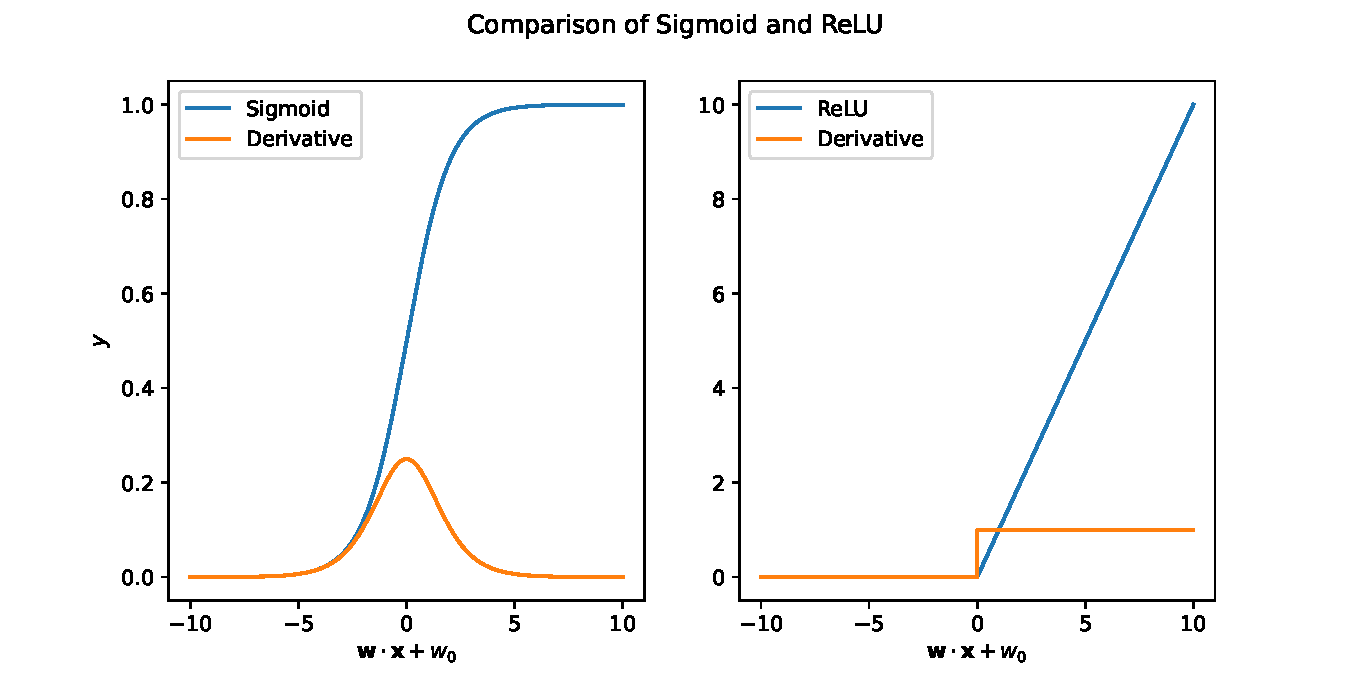
\includegraphics[width=\columnwidth]{gfx/ch3/activ.pdf}
    \caption[Activation functions]{The Sigmoid activation function compared to the ReLU, along with the respective derivatives w.r.t. the full input vector.}
    \label{fig:actfunc}
\end{figure}

There are other useful properties of the ReLu which help in the convergence of more complex models. The constant derivative helps especially to avoid the \emph{vanishing gradients} effect, where small gradients prevent the network from learning according to the algorithms presented in the next paragraph.

\paragraph{Gradient descent and backpropagation}

Now that we have devised a well suited neuron for the architecture of Figure \ref{fig:firstnn}, the objective is straightforward: \emph{find the optimal set of \emph{model parameters} (the weights) for solving the current problem.} 

Typically an \emph{objective function} or \emph{loss function} is defined, as a function
of $\mathbf{w}$, to measure how well the network with weights set to $\mathbf{w}$ solves the task. 
The objective function is a sum of terms, one for each input/target pair ($\mathbf{x}$, $\mathbf{t}$),
measuring how close the output $y$($\mathbf{x}$, $\mathbf{t}$) is to the target $\mathbf{t}$. We can denote it with $\mathcal{L}$($\mathbf{x}$, $\mathbf{t}$).

The training process is an exercise in \emph{function minimization} – i.e., adjusting $\mathbf{w}$ in such a way as to find a $\mathbf{w}$ that minimizes the objective function. Our physical intuition suggests that this might have something to do with the \emph{gradients} of the loss function. As we have already discussed, we can write the following relationship:

\[
    \Delta \mathcal{L} = \frac{\partial \mathcal{L}}{\partial \mathbf{w}} \cdot \Delta \mathbf{w} = \nabla_w \mathcal{L} \cdot \Delta \mathbf{w} 
\]
 where we have introduced the \emph{gradients vector} $\nabla_w \mathcal{L}$. If we now change the parameters at each step by an amount $ \Delta \mathbf{w} = - \eta \nabla_w \mathcal{L}$, where $\eta$ is an hyperparameter called \emph{learning rate}, we will get a corresponding change in the loss function of:
 
 \[
    \Delta \mathcal{L} = -\eta \nabla_w \mathcal{L} \cdot \nabla_w \mathcal{L} = - \eta \|  \nabla_w \mathcal{L} \|^2
\]

that is, we have updated the parameters in a way which is reducing the loss, meaning that the outputs of our network are actually getting closer to our targets--i.e. the network is \emph{learning} the optimal parameters directly from the training data! This is the idea behind \emph{gradient descent} learning algorithms, which are the current standard for training deep neural networks. The main steps are as follows:

\begin{outline}[enumerate]
    \1 Select a \emph{batch} of input/target pairs ($\mathbf{x}$, $\mathbf{t}$)$^n$ and compute the outputs \emph{y}$^n$ = \emph{f}($\mathbf{x}$, $\mathbf{t}$)$^n$;
    \1 Compute $\mathcal{L}$($y^n$), $\nabla_w \mathcal{L}^n$ and find $ \Delta \mathbf{w}^n = - \eta \nabla_w \mathcal{L}^n$;
    \1 For each batch, update the weights as $ \Delta \mathbf{w} = - \eta \sum_n \nabla_w \mathcal{L}^n$
\end{outline}

where we are assuming that the loss function may be expressed as an average of over cost functions for individual training examples. The dataset is processed multiple times as finite batches until the network reach some sort of global minimum for the loss function.

\graffito{Get an appendix for this?}
The only non trivial thing which remains to do is define the best way to compute $\nabla_w \mathcal{L}$. This can be done efficiently, with just one forward and one backward pass through the network, through the \emph{backpropagation} algorithm. Letting $\odot$ denote the \emph{elementwise} product of two vectors, we do as follows:

\begin{outline}[enumerate]
    \1 Pass the inputs through the network and get the outputs\\
    \emph{y}$^l$ = \emph{f}(\emph{y}$^{(l-1)}$) at each layer \emph{l} (feedforward pass);
    \1 Get the \emph{output error} $\delta^L = \nabla_w^L \mathcal{L} \odot y^L$:
    \1 For each previous layer, compute $\delta^l = ((w^{l+1})^T\delta^{l+1})\odot y^l$ (backward pass);
    \1 Finally, get $\nabla_w^l \mathcal{L} = \frac{\partial \mathcal{L}}{\partial w^l_{jk}} = y^{l-1}_k\delta^l_j$
\end{outline}


In practice, the loss function is monitored during training. This is usually done by evaluating it at each epoch (one full pass through the training data) on both the training data and a smaller partition reserved for testing, which the network has not seen during training. This helps to avoid \emph{overfitting}, a typical issue where the model over-optimizes for the training set, losing generalization power on previously unseen samples. This behaviour is illustrated in Figure \ref{fig:overf}.

\begin{figure}
    \centering
    \includesvg[width=\columnwidth]{gfx/ch3/2d-epochs-overfitting}
    \caption[Overfitting]{The typical behaviour of the loss (error) function during training.
    Taken from \cite{overfig}.}
    \label{fig:overf}
\end{figure}

At first, both the training and testing partition show a decrease. However, as the training goes on, the network adapts itself to the specific, stochastic features of the training data and the performance on the test partition gets worse. The dashed line is usually recognized as the best moment to interrupt training. 

\subsection{Deep Learning}
% also mention problems?
% mention residual networks?
We now know how to define efficient artificial neurons and how to combine them into networks, which can then be efficiently trained through gradient descent. 
The term \emph{deep learning} simply refers to neural networks made up of many different hidden layers, thus possessing a greater depth than most simple models. Over the years, researchers have shown how deep learning models made up of millions of parameters can actually achieve remarkable results, taking full advantage of their large number of neurons. In the following we mention some other important results which will be used through this work.

\paragraph{Residual Networks}
A great number of models and architectures have also been proposed as an alternative to the feedforward, layer-to-layer approach. A simple variation, widely adopted and also employed in the present work, is that of \emph{residual networks}, introduced by \cite{DBLP:journals/corr/HeZRS15}. The basic idea is illustrated in Figure \ref{fig:resnet}.

\begin{figure}
    \centering
    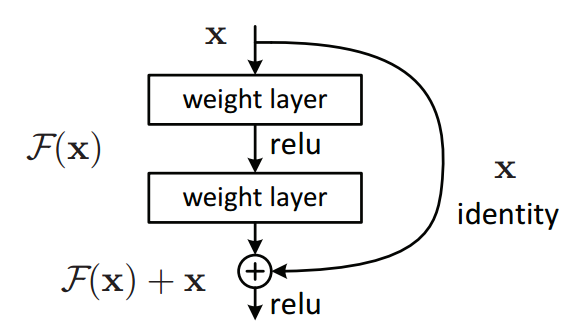
\includegraphics[width=\columnwidth]{gfx/ch3/residual.png}
    \caption[A residual block]{A residual block illustrated--taken from \cite{DBLP:journals/corr/HeZRS15}.}
    \label{fig:resnet}
\end{figure}

The idea is to define different blocks composed of one or more layers, and then to feed to the following block the input of the previous one as well as its output. Instead of hoping each stack of layers directly fits a desired underlying mapping, we explicitly let these layers fit a residual mapping. The original mapping is recast into $\mathcal{F}(x) + x$. We hypothesize that it is easier to optimize the residual mapping than to optimize the original, unreferenced mapping. To the extreme, if an identity mapping were optimal, it would be easier to push the residual to zero than to fit an identity mapping by a stack of nonlinear layers. 

This simple modification addresses a common problem in deep architectures. When the model saturates the problem, it starts to overfit, especially in later layers; by defining a residual block we may simply allow the network to learn an identity mapping and avoid the issue.

\paragraph{Batch Normalization}
\emph{Batch normalisation} normalises a layer input by subtracting the batch mean and dividing it by the batch standard deviation, while defining a \emph{scale} and a \emph{shift} parameters for each neuron to avoid losing representation power due to this rescaling of the inputs. The method was first introduced in \cite{https://doi.org/10.48550/arxiv.1502.03167}, and it has been tested in a large variety of models, proving that it is an effective way of contrasting common training instabilities and for speeding up convergence.

\paragraph{Cosine Annealing}
Cosine Annealing is a type of learning rate schedule that has the effect of starting with a large learning rate that is relatively rapidly decreased to a minimum value before being increased rapidly again. The resetting of the learning rate acts like a simulated restart of the learning process and the re-use of good weights as the starting point of the restart is referred to as a \emph{warm restart} in contrast to a \emph{cold restart} where a new set of small random numbers may be used as a starting point. The proper formula its:

\[\eta_{t} = \eta_{min} + \frac{1}{2}\left(\eta_{max}-\eta_{min}\right)\left(1+\cos\left(\frac{T_{cur}}{T_{max}}\pi\right)\right)\]

were $\eta$ is the learning rate and $T$ the training epoch.
It was introduced by \cite{https://doi.org/10.48550/arxiv.1608.03983}.

The training and the convergence of deep learning models is also plagued by others problems, making the training of complex models somewhat of an empirical process. We limit ourselves to mentioning the most relevant issues for our use-case in the following section.

\section{Generative Models} 

A well developed subset of deep learning models, \emph{Generative models} are a class of architectures which aim to produce novel and original samples similar to the ones presented during training, usually starting from randomly distributed noise. The most well know use case is the field of \emph{image generation}, and two specific architectures are the most widely adopted.

\subsection{State of the art}

\paragraph{Generative Adversarial Networks}

Introduced by Goodfellow et al. \cite{gan}, Generative Adversarial Networks (GANs for short) are a framework for training powerful generative models. Two neural networks contest with each other in a game (in the form of a zero-sum game, where one agent's gain is another agent's loss): the generative network G learns to map from a latent (usually gaussian) noise space to a data distribution of interest, while the discriminator network D distinguishes candidates produced by the generator from the true data distribution. G's training objective is to increase the error rate of D by producing samples so close to the target that D misclassifies them consistently as coming from the real samples. The framework is illustrated in Figure \ref{fig:gan}.


\begin{figure}
    \centering
    \scalebox{0.90}{
    \begin{tikzpicture}[
        ->, thick,
        node/.style={circle, fill=teal!60},
        label/.style={below, font=\footnotesize},
      ]
    
      \node[node] (zin) {$\vec z_\text{in}$};
      \node[node, right=5em of zin] (fake) {$\vec x_\text{fake}$};
      \draw (zin) -- node[above] {$G(\vec x)$} node[label] {generator} (fake);
    
      \draw[<-] (zin) -- node[above] {$p_\theta(\vec z)$} node[label] {latent noise} ++(-3,0);
      \node[node, above=of fake] (real) {$\vec x_\text{real}$};
      \draw[<-] (real) -- node[above] {$p_\text{data}(\vec x)$} ++(-3,0);
      \node[node, right=6em of fake] (D) at ($(fake)!0.5!(real)$) {$\vec x$};
      \node[right=7em of D] (out) {real?};
      \draw (D) -- node[above] {$D(\vec x)$} node[label] {discriminator} (out);
    
      \coordinate[right=2.5em of fake, circle, fill, inner sep=0.15em] (pt1);
      \coordinate[right=2.5em of real, circle, fill, inner sep=0.15em] (pt2);
    
      \draw[-, dashed] (pt1) edge[bend left] coordinate[circle, fill=orange, inner sep=1mm, pos=0.7] (pt3) (pt2);
      \draw (fake) -- (pt1) (real) -- (pt2) (pt3) -- (D);
    
    \end{tikzpicture}}
    \caption[GAN]{The GAN training framework illustrated.}
    \label{fig:gan}
\end{figure}

\paragraph{Variational Autoencoders}

The main idea behind the \emph{Variational Autoencoder} (VAE) architecture, theorized by Kingma et al \cite{vae}, is to employ a network made up of two parts: the \emph{encoder} and the \emph{decoder}. The encoder learns to map input data to a set of parameters $\pmb{\mu}$ and $\pmb{\sigma}$, which together make up a \emph{latent} Gaussian representation $\mathbf{z}$. The decoder is trained to scale up the parameters from the new latent space back to the original training space.

The network is trained to correctly encode and decode the data, and once trained the decoder may receive as input random Gaussian noise and produce new original samples. The idea is illustrated in Figure \ref{fig:vae}.

\begin{figure}
    \centering
    \scalebox{0.65}{
    \begin{tikzpicture}[
        shorten >=1pt, shorten <=1pt,
        neuron/.style={circle, draw, minimum size=4ex, thick},
        legend/.style={font=\large\bfseries},
      ]
    
      % encoder
      \drawNodes{encoder}{{{,,,,}, {,,,}, {,,}}}
      \denselyConnectNodes{encoder}{{5, 4, 3}}
    
      % decoder
      \begin{scope}[xshift=11cm]
        \drawNodes{decoder}{{{,,}, {,,,}, {,,,,}}}
        \denselyConnectNodes{decoder}{{3, 4, 5}}
      \end{scope}
    
      % mu, sigma, sample nodes
      \foreach \idx in {1,...,3} {
          \coordinate[neuron, right=2 of encoder-3-2, yshift=\idx cm,, fill=yellow, fill opacity=0.2] (mu-\idx);
          \coordinate[neuron, right=2 of encoder-3-2, yshift=-\idx cm, fill=blue, fill opacity=0.1] (sigma-\idx);
          \coordinate[neuron, right=4 of encoder-3-2, yshift=\idx cm-2cm, fill=green, fill opacity=0.1] (sample-\idx);
        }
    
      % mu, sigma, sample boxes
      \node [label=$\pmb{\mu}$, fit=(mu-1) (mu-3), draw, fill=yellow, opacity=0.45] (mu) {};
      \node [label=$\pmb{\sigma}$, fit=(sigma-1) (sigma-3), draw, fill=blue, opacity=0.3] (sigma) {};
      \node [label=$\pmb{z}$, fit=(sample-1) (sample-3), draw, fill=green, opacity=0.3] (sample) {};
    
      % mu, sigma, sample connections
      \draw[->] (mu.east) edge (sample.west) (sigma.east) -- (sample.west);
      \foreach \a in {1,2,3}
      \foreach \b in {1,2,3} {
          \draw[->] (encoder-3-\a) -- (mu-\b);
          \draw[->] (encoder-3-\a) -- (sigma-\b);
          \draw[->] (sample-\a) -- (decoder-1-\b);
        }
    
      % input + output labels
      \foreach \idx in {1,...,5} {
          \node[left=0 of encoder-1-\idx] {$x_\idx$};
          \node[right=0 of decoder-3-\idx] {$\hat x_\idx$};
        }
      \node[above=0.1 of encoder-1-1] {input};
      \node[above=0.1 of decoder-3-1] {output};
    
    \end{tikzpicture}}
    \caption[VAE]{The Variational Autoencoder illustrated.}
    \label{fig:vae}
\end{figure}

\subsection{Known issues}

This two architectures have achieved remarkable results. However, there are still many issues related to their applicability. The following is a brief and incomplete list:

\begin{outline}
    \1 GANs are affected by numerous training instabilities, as their peculiar training system must be carefully engineered to avoid that one of the two agents surpasses the other too much too fast, thus invalidating the training;
    \1 GANs are also plagued by  \emph{mode collapse}, where the generator over-optimizes for a particular discriminator, and the discriminator never manages to learn its way out of the trap. As a result the generators rotate through a small set of output types, degrading the statistical significance of generated samples;
    \1 VAEs with Gaussian latent distributions are generally noisy. VAEs are poor models of data whenever insufficiently flexible latent distributions are used--that is, distributions which do not reflect the underlying data distribution. Usually the Gaussian distribution is an approximation at best, making the results sub-optimal;
    \1 More generally, almost all of the model in the literature are usually geared towards the task of image generation and recognition. This type of architectures often perform poorly when simply re-adapted to the HEP use case, which typically consists of lower dimensional, sparse data structures. 
\end{outline}

Both GANs and VAEs have already been extensively investigated by the collaborations at CERN (see \cite{2019glhc} and \cite{otten2021event}); despite this, there is still a limited literature regarding behavior in low dimensionality as in our case, e.g. \cite{523096}.

Fortunately, there exist another type of latent generative model, which, despite being definitely less popular than the ones already discussed, is more well suited to our application and makes up the backbone of the present work. We thus turn to the following chapter for a more in depth discussion.
% low dim paper?

%*****************************************
%*****************************************
%*****************************************
%*****************************************
%*****************************************
